%% EU ICT Proposal LaTeX template
%% V1.0
%% Based on the h2020proposal.cls LaTeX class for writing EU H2020 RIA proposals.
%% 
%% Copyright (c) 2010, Giacomo Indiveri
%%
%%  This latex class is free software: you can redistribute it and/or modify
%%  it under the terms of the GNU General Public License as published by
%%  the Free Software Foundation, either version 3 of the License, or
%%  (at your option) any later version.
%%
%%  h2020proposal.cls is distributed in the hope that it will be useful,
%%  but WITHOUT ANY WARRANTY; without even the implied warranty of
%%  MERCHANTABILITY or FITNESS FOR A PARTICULAR PURPOSE.  See the
%%  GNU General Public License for more details.
%%
%%  You should have received a copy of the GNU General Public License
%%  along with h2020proposal.cls.  If not, see <http://www.gnu.org/licenses/>.
%%
%% Contributors: Elisabetta Chicca
%%
%% Disclaimer: The template is based on the document provided by the EU Participants Portal 
%% h2020-call-pt-ria-ia_en, Version 1.4, 21 May 201
%%
%% Use the original source and the http://ec.europa.eu/ documentation for reference. We make no
%% representations or warranties of any kind, express or implied, about the completeness, accuracy,
%% reliability, suitability or availability with respect to the original template.
%% In no event will we be liable for any loss or damage including without limitation, indirect or
%% consequential loss or damage, or any loss or damage whatsoever arising out of, or in connection
%% with, the use of this template and/or class.
%%
%% Makes use of the memoir class. Read the optimum memman documentation for
%% info on how to customize your proposal.


\documentclass[]{h2020proposal}     % Remove 'draft' option for final version
%\documentclass[draft]{h2020proposal} % Use 'draft' option to show comments and labels

% For in-line comments use:
% \marginpar{comment text}

%% Extra Packages
%% ========
%\usepackage{fontspec}% Latin Modern by default with xelatex

%% LaTeX Font encoding -- DO NOT CHANGE
\usepackage[OT1]{fontenc}

%% Input encoding 'utf8'. In some cases you might need 'utf8x' for
%% extra symbols. Not all editors, especially on Windows, are UTF-8
%% capable, so you may want to use 'latin1' instead.
%\usepackage[utf8,latin1]{inputenc}
\usepackage[utf8x]{inputenc}
\usepackage{lmodern,textcomp}

%% Babel provides support for languages.  'english' uses British
%% English hyphenation and text snippets like "Figure" and
%% "Theorem". Use the option 'ngerman' if your document is in German.
%% Use 'american' for American English.  Note that if you change this,
%% the next LaTeX run may show spurious errors.  Simply run it again.
%% If they persist, remove the .aux file and try again.
\usepackage[english]{babel}

%% For underlined wrapped text.
\usepackage{soul}

%% This changes default fonts for both text and math mode to use Herman Zapfs
%% excellent Palatino font.  Do not change this.
\usepackage[sc]{mathpazo} % Not needed with xelatex

%% The AMS-LaTeX extensions for mathematical typesetting.  Do not
%% remove.
\usepackage{amsmath,amssymb,amsfonts,mathrsfs}

%% Gantt Charts in LaTeX
\usepackage{pgfgantt}

%% LaTeX' own graphics handling
\usepackage{graphicx}

%% Fancy character protrusion.  Must be loaded after all fonts.
\usepackage[activate]{pdfcprot}

%% Nicer tables.  Read the excellent documentation.
\usepackage{booktabs}

% Compressed itemized lists (with a * at the end)
\usepackage{mdwlist}

%% Nicer URLs.  
\usepackage{url}

\usepackage{wrapfig}

\usepackage{siunitx}
\sisetup{
  group-four-digits = true,
  group-separator = {\ },
%  output-decimal-marker = {,},
%  round-integer-to-decimal,
%  round-precision = 2,
  round-mode=places,
  detect-weight=true,
  detect-family=true,
}

\usepackage{subfiles}
\newcommand{\onlyinsubfile}[1]{#1}
\newcommand{\notinsubfile}[1]{}

%% Configure citation styles
\usepackage[numbers,sort&compress,square]{natbib}
\def\bibfont{\footnotesize}     %for smaller fonts in the biblio section

%% Hyper Ref package. In order to operate correctly, it must be the last package declared
\usepackage[colorlinks,pagebackref,breaklinks]{hyperref} 

%% Euro sign
\usepackage{eurosym}

\usepackage{tabularx}
% Wrap and center
\newcolumntype{Y}{>{\centering\arraybackslash}X}

\usepackage{colortbl}
\usepackage{float}

\usepackage{pdfpages}

\usepackage{titlesec}

% Used on Figures of Positioning of the Project
\usepackage{caption}
\usepackage{subcaption}

\titleformat
{\chapter} % command
[display] % shape
{\bfseries\Large\itshape} % format
{\vspace{-15ex}} % label
{0pt} % sep
{\thechapter~} % before-code
[
\vspace{-5ex}%
] % after-code


%\titleformat{\chapter}[display]
%  {\normalfont\Huge\bfseries}{}{}{\thechapter~\Huge}
%\titlespacing*{\chapter}{0pt}{-15pt}{20pt}
%\titlespacing*{name=\chapter,numberless}{0pt}{-15pt}{10pt}

%\makeatletter
%\renewcommand{\@makeschapterhead}[1]{%
%  \vspace*{50\p@}%
%  \vspace*{0\p@}%
%  {\parindent \z@ \raggedright
%    \normalfont
%    \interlinepenalty\@M
%    \large \bfseries  #1\par\nobreak
%    \vskip 40\p@
%    \vskip 10\p@
%  }}
%\makeatother

%% Extra package options
\hypersetup{
  hypertexnames=true, linkcolor=blue, anchorcolor=black,
  citecolor=blue, urlcolor=blue  
}

\urlstyle{rm} %so it doesn't use a typewriter font for urls.
\DeclareGraphicsExtensions{.jpg,.pdf,.mps,.png} % for pdflatex
\graphicspath{{img/} {./}} %put all figures in these dirs

\newcommand{\alert}[1]{{\color{red}\textbf{#1}}}

%%%%%%%%%%%%%%%%%%%%%%%%%%%%%%%%%%%%%%%%%%%%%%%%%%%%%%%%%%%%%%%%%%%%%%

%% ========================================================
%% IMPORTANT store proposal information in global variables
%% ========================================================
\title{iWe: Social cloud computing}
\shortname{iWe} 
\titlelogo{}{0.25} % file name and scale
\fundingscheme{Research and Innovation Action}
\topic{Work Programme topic addressed}
\coordinator{Peter Senna Tschudin}{peter.senna@gmail.com}{+41767614456}
\participant{iWe}{iWe}{Switzerland} % First participant is the coordinator
%\participant{University of partner 2}{UoP2}{Country2} % as example...
%\participant{University of partner 3}{UoP3}{Country3} % as example...
% etc.

% Page Headers
%\makeoddhead{proposal}{\disptoken{@acronym}}{}{\rightmark}
%\makeevenhead{proposal}{\leftmark}{}{\disptoken{@acronym}}

%Page Footers
%\makeevenfoot{proposal}{ \thepage }{ \date{\today} }{ \disptoken{@acronym} }
%\makeoddfoot{proposal}{  }{ \date{\today} }{ \thepage }

%Page Style
\pagestyle{proposal} %use \pagestyle{showlocs} for debugging

%Heading style 
\makeheadstyles{default}{%
\renewcommand*{\chapnamefont}{\normalfont\bfseries}
\renewcommand*{\chapnumfont}{\normalfont\bfseries}
\renewcommand*{\chaptitlefont}{\normalfont\bfseries}
\renewcommand*{\secheadstyle}{\normalfont\bfseries}
}%
\headstyles{default}

%Chapter Style
\chapterstyle{section} %Avoid writing the word "Chapter" at the beginning of each proposal section
% other possible valid styles:
% article, bringhurst, crosshead, culver, dash, demo2, ell, southall, tandh, verville, wilsondob
\renewcommand*{\chaptitlefont}{\normalfont\Large\bfseries}
\renewcommand*{\chapnumfont}{\normalfont\Large\bfseries}


%\linespread{0.9}

\begin{document}
\renewcommand{\onlyinsubfile}[1]{}
\renewcommand{\notinsubfile}[1]{#1}

%% TITLE
\maketitle

\vspace{-1em}
\renewcommand\contentsname{Table of Contents}
\setlength{\cftbeforechapterskip}{1.0em plus 0.3em minus 0.1em}
\renewcommand{\cftchapterbreak}{\addpenalty{-4000}}
%\makeparticipantstable
\tableofcontents*              
%\input{abstract}              
\pagebreak


%% Main proposal

%% Fixed proposal structure - Do not change
%%% Important. To have correct table numberings
\renewcommand{\thetable}{\thesection\alph{table}}

\chapter{Excellence}
\label{cha:excellence}

%More than a decade after Amazon introduced public cloud services, common sense
%is that consuming public cloud services is more economical than having internal
%IT. However this comparison is a distraction, as the proper question is
%\textbf{can your internal IT be as economical as Amazon's internal IT}?
%
%The real revolution that Amazon introduced in 2006 was not offering public cloud
%services, but rather \textbf{offering public cloud services to offload the costs
%of their internal IT}. Amazon was looking for a solution to a complicated
%problem: how to meet the widely varying load requirements of Amazon's virtual
%store and reduce operational costs at the same time. Offering public cloud
%services allowed Amazon to have resources for peak load demands, and to hire out
%idle resources reducing operational costs.
%
%If you believe you can save by using Amazon cloud services, imagine the
%possibilities of \textbf{following Amazon's steps and offloading the costs of
%your internal IT}. \textit{iWe} is offering a revolutionary service that
%combines the convenience and flexibility of a public cloud, performance,
%control, and privacy of internal IT, with Amazon's cost offloading strategy. Our
%customers get the best of public clouds, the best of internal IT, and
%unprecedented economy. We estimate savings for an SME of a factor of 5 compared
%to public cloud, and of a factor of 15 compared to traditional internal IT.

More than a decade after Amazon introduced public cloud services, common sense
is that consuming public cloud is more economical than having internal IT.
However this comparison is a distraction that shows public clouds in a favorable
light. The question we are going to help you answer is \textbf{can your internal
IT be as economical as Amazon's internal IT}?

The real revolution that Amazon introduced in 2006 was offering public cloud
services \textbf{to offload the costs of their internal IT}. Amazon was looking
for a solution to a complicated problem: how to meet the widely varying load
requirements of Amazon's virtual store and reduce operational costs at the same
time. Amazon's virtual store peak capacity is hard to predict, and purchasing
servers and data center gear for peak load would be inefficient most of the
time. Offering public cloud services allowed Amazon to have resources for peak
load demands of their virtual store, and to hire out idle resources reducing
operational costs.

If you believe you can save by consuming Amazon cloud services, imagine the
possibilities of \textbf{offloading the costs of your internal IT}.
\textit{iWe} is offering a revolutionary service that combines the
convenience and flexibility of a public cloud, performance, control, and privacy
of internal IT, with Amazon's cost offloading strategy. Our customers get the
best of public clouds, the best of internal IT, and unprecedented economy. We
estimate savings for an SME of a factor of 5 compared to public cloud, and of a
factor of 15 compared to traditional internal IT.

\section{Objectives}
\label{sec:objectives}

% Internet has become an engine for innovation, economic growth, job creation
% and social progress. It is accelerating innovation, reshaping established
% industries, facilitating new ways of doing business, and transforming social
% behaviours. At the same time, this increasing diversification of usage
% patterns and of applications, is posing stronger requirements on the
% underlying networking and computing infrastructures.

Our objective is to do a low cost validation of our new approach to cloud
computing by doing a small scale deployment of our prototype. We will host
copies of existing popular Internet services such as Wikipedia and
Stackoverflow, for simulating real world loads, and compare it to existing
providers. We want to know how many users we can serve with the infrastructure
of our small scale deployment, and at which cost per user.  We will measure and
collect all sorts of technical and commercial parameters that are essential for
our business plan.

\section{Concept}
\label{sec:concept}

\begin{figure}
    \centering
    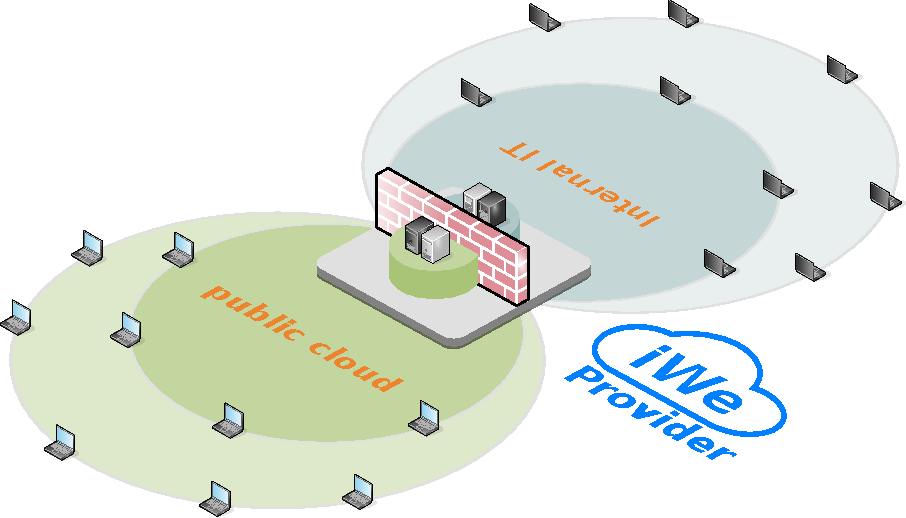
\includegraphics[width=0.7\textwidth]{images/iwe-providers-consumers-with-template2.pdf}
    \caption{SME \textit{iWe Provider}}
    \label{fig:the-clalld-pvt-pub}
\end{figure}

While Internet is becoming essential in virtually all areas of human activities,
cloud computing is pushing Internet away from servers we used to own and
control. One negative result of migrating to the cloud is Internet
centralization, with a few very powerful companies privately owning major shares
of the hardware, software and networks that runs the Internet and stores
\textbf{our} data. With the unbalance between massive providers and
comparatively small consumers, we subject ourselves to services that are
essential to our personal and professional activities, but that may lack
transparency, privacy, control, performance, and a fair price.

We are creating a better cloud, but instead of joining the race for Internet
ownership, instead of building our own massive data centers, we are reverting
the Internet centralization trend by empowering companies (and later will also
empower individuals) from cloud consumers to cloud providers. Our focus on
empowering our community comes from our open source attitude. We are an open
source company, and we are pushing open source ideas to new levels, which is
allowing us to create the first cloud computing sharing economy.

\textit{iWe} will pioneer the sharing economy for cloud computing in a
similar fashion to what Uber does with transport, and to what Airbnb does with
housing. We will start offering public cloud services that are provided by our
community of \textit{iWe Providers} who are the equivalent of Uber drivers,
and Airbnb hosts.

We welcome \textit{iWe Providers} to join us purely for profit, but we expect
to maximize our impact with a different user profile. We expect SMEs to use our
services to get cloud computing resources for their own use, but in better terms
with a transparent service that guarantees technological independence, privacy,
control, performance, and excellent savings. We are confident in our popularity
among SMEs because we offer levels of IT efficiency, convenience, privacy,
and performance that were not previously available to them. We expect SMEs to
use our services to be more competitive, by reducing IT costs, and by getting
more connected computing resources.

As an example, we will describe an SME that joins our community of
\textit{iWe Providers} to get cost-efficient cloud resources for their own
use. This SME has modest needs: 128 GB of RAM, 1000 GB of storage with N+1
redundancy. We opted to demonstrate such as small configuration as we consider
it to be a challenging scenario for efficiency, while common for SMEs
world-wide. Our proposed architecture for this SME is shown on Figure
\ref{fig:the-clalld-pvt-pub} with four physical servers, in two redundancy
pairs, each pair targeting a different audience. The servers run our software
stack which allows us to assume the maintenance responsibility of the entire
environment.

Maintaining the servers of our \textit{iWe Providers} result in a major
advantage: the skills \textit{iWe Providers} need to manage and maintain
their IT lie on the realm of the \textbf{power user} and not the seasoned IT
administrator. As we will show on Table \ref{table:clouds-comparison} of Section
\ref{sec:expected-impact} not requiring systems engineers to maintain the
environment can reduce IT costs.  \textit{iWe} also takes full responsibility
over the public cloud services that we offer but that are provided by our
community of \textit{iWe Providers}. \textit{iWe Providers} don't need to
interact with and worry about consumers for their surplus of server capacity,
and public cloud consumers get a consistent consumer experience from
\textit{iWe}.

Figure \ref{fig:the-clalld-pvt-pub} shows the smallest possible configuration
for an efficient Internal IT capable of high availability, and cost offloading.
The servers on the Internal IT circle are used exclusively by the SME
\textit{iWe Provider} for applications and data that are sensitive in term of
privacy or performance. The other two servers on the public cloud circle provide
the means for offloading costs of the \textit{iWe Provider}. Cost offloading
works in two ways: capacity of these servers is sold as public cloud services on
the \textit{iWe} marketplace and the income is transferred to the SME
\textit{iWe Provider}, and the SME \textit{iWe Provider} can also consume
public cloud resources avoiding additional expenses.

Another characteristic of our service is that we do not charge money from the
\textit{iWe Providers}. Not charging money for our Internal IT service is
core to \textit{iWe} business model, but it doesn't make it a free service.
Instead of charging fees, we exchange our Internal IT service for a share of the
connected computing resources we maintain. This strategy keep the operational
costs low for the \textit{iWe Providers} and give us a building block for our
public cloud services. We sell public cloud services for a profit on our
marketplace closing the loop with income for us.

Our paid public cloud services will start offering regular IaaS with storage,
virtual machines and containers, but with two major advantages: we will offer
extended control over geographical location of resources, allowing deployment in
cities and neighborhoods (instead of continents and countries of current
providers), and the cost structure of \textit{iWe} is efficient. Our business
model allows us to have a massive distributed public cloud without expenses we
would have with traditional data centers. We offload to \textit{iWe
Providers} costs with servers, data center gear, and utility bills, making our
cost structure very efficient.

\section{Positioning of the project}
\label{sec:positioning}

\begin{figure}
\centering
\begin{subfigure}{.5\textwidth}
  \centering
  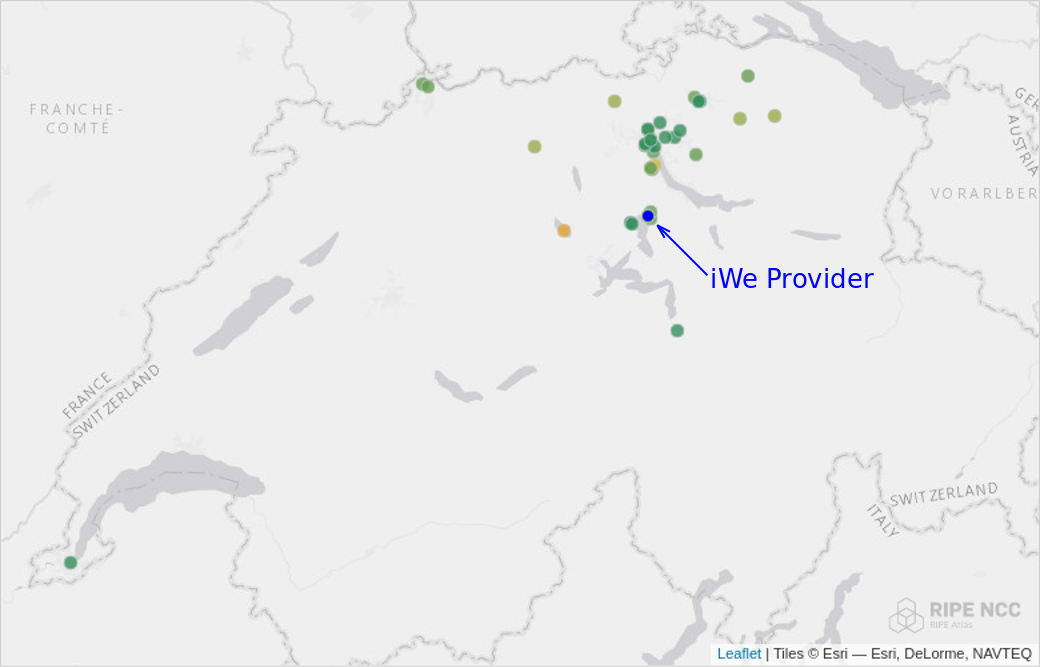
\includegraphics[width=0.98\textwidth]{images/atlas-map.png}
  \vspace{-0.05in}
  \caption{Where are we pinging from}
  \vspace{0.1in}
  \label{fig:sub1}
\end{subfigure}%
\begin{subfigure}{.5\textwidth}
  \centering
  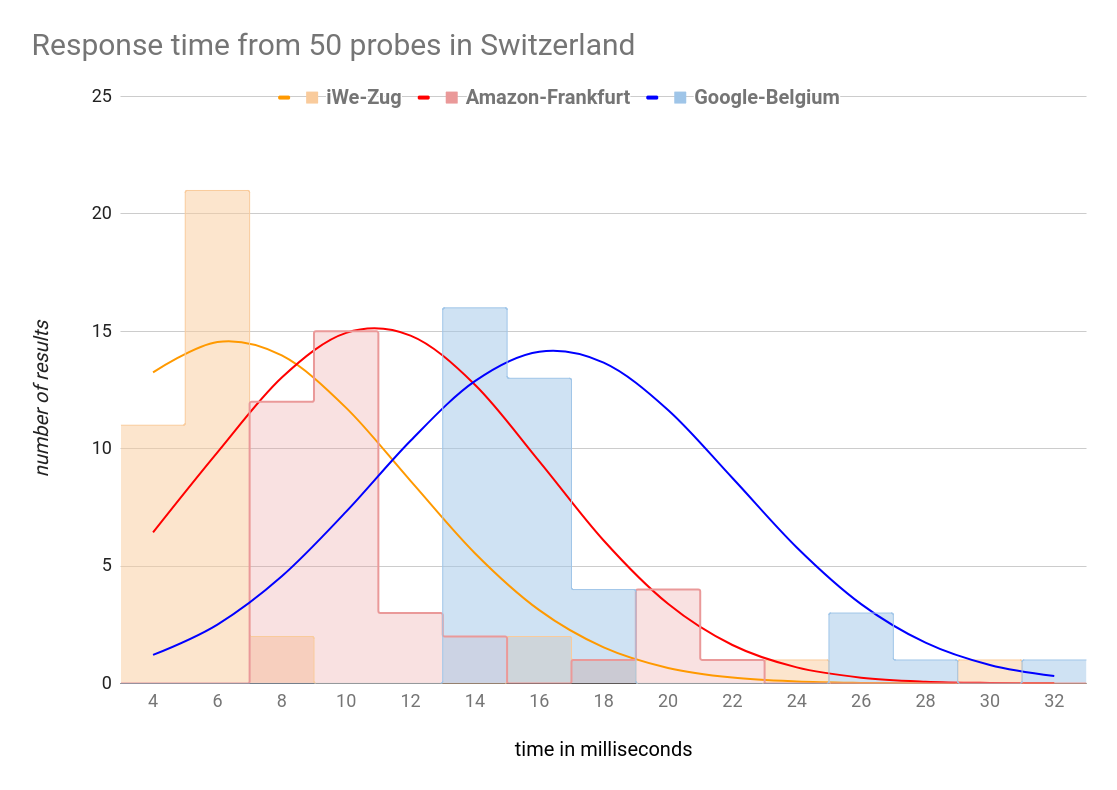
\includegraphics[width=0.96\textwidth]{images/response-time-50.png}
  \vspace{-0.05in}
  \caption{Ping normal distribution and histogram}
  \vspace{0.1in}
  \label{fig:sub2}
\end{subfigure}
  \caption{Details about our latency test}
  \label{latency}
\end{figure}

\begin{table}
    \centering
    \begin{tabular}{r l l l}
                                    & Amazon EC2     & Google Compute & iWe \\
        \hline
        Instance type               &  t2.large & n1-standard-2 & - \\
        \hline

        vCPUs                       &  2 & 2 & 2 \\
        \hline

        Memory                      & 8GB & 7.5GB & 7.5GB \\
        \hline

        Disk                        & 80GiB & 80GB &  80GiB \\
        \hline

        Disk Type                   & GP2 & SSD persistent & SSD persistent \\
        \hline

        Zone                        & eu-central-1b & europe-west1-c & zug-1 \\
        \hline

        Location                    & Frankfurt & Belgium & Zug \\
        \hline

        Monthly cost                & \$ 107.95 & \$ 41.55 & TBD \\
        \hline
    \end{tabular}
    \caption{Specification of the instances}
    \label{table:instances}
\end{table}

We compared the performance of instances running in a very small iWe
provider to instances from Amazon and Google. Table \ref{table:instances} shows
the configuration of each instance, and cost forecast from Amazon and Google.

For Google and Amazon we selected the zones with the lowest latency and higher
bandwidth to our test site in Zug. We used the Network speed test from
CloudHarmony\footnote{https://cloudharmony.com/speedtest-for-aws,
https://cloudharmony.com/speedtest-for-google} to find the zones with better
network performance. All the instances run the same software stack, from the
kernel to the benchmark tools.

We were pinging the instances from 50 different locations in Switzerland as
shown by Figure \ref{latency}(a). Figure \ref{latency}(b) shows the distribution
of results with 82\% of response times for iWe provider in Zug being under 6 ms.
We are using probes from the Ripe Atlas
project\footnote{https://atlas.ripe.net/api/v2/measurements/groups/9229432/} for
our latency test. Figure \ref{graphs}(c) shows the geometric mean of response
times from the probes we are using.

Section \ref{cha:appendix} contains detailed benchmark results for CPU, memory
and IO.

We now plan to extend this benchmark to 10 different locations in Zug,
Switzerland covering different use cases. However full commercialization of
\textit{iWe} will require creation and polishing of web interfaces, server
images, and back end infrastructure.

\section{Methodology}
\label{sec:methodology}

% Describe what you want to achieve in the feasibility assessment. Explain the
% methodology, distinguishing, as appropriate, activities linked to assess the
% technological/technical/practical feasibility and economic viability (e.g.
% market studies, customer survey, etc.).

The next step is to do a deployment of 10 small sites in Zug, Switzerland. Each
site will contain four physical servers connected to the Internet, and running
our software stack. The main idea is to evaluate the real value of the added
granularity of 10 locations in Zug compared to large data centers in Zurich and
Germany.

For an increased commercial impact, we will discuss in details on Section
\ref{sec:expected-impact} our plans to design, build, and sell unique high end
low cost servers for our customers, but for the feasibility assessment we are
going for the simplest and cheapest solution: refurbished notebooks. Our target
notebook is the 14" Lenovo Thinkpad T430 equipped with 16 GB of RAM, 2X 1TB SSD,
an i5-3320M CPU, and a 4G modem we can use as a backup communication channel.
Our hardware partner from Germany currently has 900+ units ready for delivery,
each unit priced just under 400,00 €. We are going to buy 40 notebooks for 10
sites with 4 notebooks each.

The total \textit{cloud power} of our small scale deployment will be distributed
in 10 locations, providing 40 TB of redundant storage, 640 GB of RAM memory, and
160 CPU threads. While our entire cloud is smaller than a single modern server,
we have enough resources for our tests. We can, for example, host more than 300
copies of the entire Wikipedia, or 140 copies of latest version of the massive
network of Stackoverflow sites.

The main question we are going to answer with out 10 sites test deployment is
the real value of the increased granularity of having 10 providers in Zug
compared to having larger centralized providers in Zurich and in Germany. We
want also to find out how many users we can serve, and at which cost per user.
We also need to test Content Delivery Network (CDN), functionality to experiment
with our extended granularity. After we are done with the laboratory tests we
will invite early adopters to test non-critical loads on our infrastructure,
which we expect to provide additional valuable input for our business plan.

\section{Ambition}
\label{sec:ambition}

% Explain the novelty of your innovation business project. What do you envisage
% as key market application of the innovation project result?

Section \ref{sec:concept} covered high level overview of the novelty of our
innovation project, key market applications, and the envisaged solution. This
section will describe our potential, and why it is worth to develop and invest
in \textit{iWe}. We will describe opportunities with IoT, the strategy for
our market places, how we plan to gain global traction with local Internet
providers, describe our target relationship with Telecommunication
Companies(Telecoms), and describe our future expansion with home users.

\textbf{IoT} - Peter Levine from Andreessen Horowitz mentioned in a recent
podcast \cite{the-end}: \textit{Cloud computing has pushed computation away from
our own private servers resulting in performance issues related to high latency
between the client and the cloud server. As IoT proliferates, the current model
of cloud computing will become too slow. A small difference in the time it takes
to get a response from the cloud server could be the difference between life and
death in automation for cars and drones.  Computation will move to the edge. In
such an edge computing model, there will be trade of computational resources
without any request to a centralized cloud server.} In the \textit{iWe}
context this excerpt describes how our decentralized architecture will meet IoT
requirements gracefully, as we offer connected computing resources on the edges
of the network, and as we offer a framework for using connected computing
resources as a currency for trade.

\textbf{Marketplaces} - We will have two interconnected marketplaces. The
consumer marketplace is a traditional e-commerce platform that will generate
most of our income by offering services and goods provided by \textit{iWe}
and partners. The services and goods that the consumer marketplace will offer
are defined by our second marketplace, the trusted partner marketplace. We will
offer \textit{iWe} infrastructure and community resources as building blocks
for our partners to create new services, but we will also allow our partners to
create their own customized building blocks. We expect this flexibility to
attract partners that can take advantage of the extended control that
\textit{iWe} offers over the lower software layers of their cloud solution
stack.  As examples, we expect companies such as VMWare, Citrix, SAP, Oracle,
Microsoft, Suse, and Red Hat to offer various services through our trusted
partner marketplace.

\textbf{Global traction} - We offer great cloud solutions to SMEs of all kinds,
but we will start by targeting a specific market niche: Local Internet Service
Providers (LISP). Local means that their service offer is limited to a
geographical area, which is common to providers of Internet access, and of data
center services, such as hosting and co-location. LISPs were popular before cloud
computing, but they are having a hard time competing with giants such as Amazon
and Google. We can help them to regain competitiveness, and to increase revenue
with little effort.  LISP already have the physical infrastructure, including
servers and Internet connection, which will make their gradual transition to
\textit{iWe Providers} easy and cheap. We see LISPs as key partners worldwide
during our first steps on the market.  We will focus on making them an important
share of our early adopters.

\textbf{Telecoms} - With the Internet moving to a few massive data centers, the
role of Telecommunication Companies is rapidly changing from Internet providers
to Internet consumers. One important factor is the loss of corporate customers
to the cloud, which represents services migrating from the Telecom network to
the cloud. One may argue that cloud computing can bring new customers to
Telecoms, however the cloud only brings consumers of the same massive data
centers that were already forcing Telecoms into Internet consumers, speeding up
the transition.  \textit{iWe} offers a shift to the trend of relevance loss,
giving even SMEs the power to host their own services, avoiding moving them to
the cloud or moving them back to the network of their (or our) favorite Telecom.
We also believe we can help Telecoms to sell more connectivity services, and we
expect to develop good partnership with Telecoms worldwide by offering them
highlighted visibility on our marketplaces.

\textbf{The future at home} - We know that enabling individuals to do business
is a powerful strategy that giants such as Uber and Airbnb implement very well.
We want to offer home users a simple way to add resources to the Public
\textit{iWe} for a profit, and expect them to considerably increase our
granularity to support our offer of cloud resources in neighborhoods around the
globe.  We also want to extend the idea of using connected computing resources
as currency for online services, offering \textit{Home iWe Providers}
attractive services to spend their connected resources, instead of simply
trading it all for cash. An example would be to get a premium subscription from
Netflix in exchange for cloud services.
 % Section I
\vspace{10ex}
\chapter{Impact}
\label{cha:impact}

\section{Expected impacts} 
\label{sec:expected-impact}


We will empower even small companies to offload the costs of their internal IT,
and gain technological independence over their connected computing resources.
\textit{iWe} is basically identifying and fixing gaps in cloud efficiency that
SMEs can't currently avoid.  In this section we will briefly describe our Total
cost of ownership (TCO) analysis, our powerful internal IT architecture, the
potential we have to save up to 50\% in power consumption, and how we plan to
further reduce costs for our customers designing, building, and selling our own
cloud hardware.

\subsection{Internal IT powered by \textit{iWe}} 
\label{subsec:iitic}

In the past the minimum possible setup for a reliable and flexible internal IT
would include two servers for redundancy and a storage device that also offers
redundancy. The need of a storage device adds complexity, increase acquisition
costs and complicates maintenance.  The storage is needed to physically separate
data from servers, allowing a key technical feature named \textit{live
migration}.

\textit{Live migration} is a feature that allows to move virtual machines, and
other resources, between different physical servers, \textbf{while the resources
are running}, and without noticeable interruption. It is extremely valuable for
maintenance and for fault tolerance, and the lack of \textit{live migration} is
not acceptable.

Using the \textit{iWe} server architecture the minimum possible setup uses
only two servers, and there is no need for a dedicated storage device. Instead
of physically separating data from servers, instead of using an external and
shared storage device, we keep the data synchronized on multiple servers, saving
one copy of the data on each server.  This design allows for \textit{live
migration} at a fraction of complexity and costs. While this is not the best
configuration for large scenarios, it is clearly more efficient for environments
with small server count.

We tested the performance (bandwidth and latency) of our synchronization
technique on SSD disks, and the results were positive. We could reach
native SSD speeds with marginal increase in CPU load, suggesting that our
synchronization mechanism offer performance increase over entry level storage
devices that are popular for SMEs.

The \textit{iWe} server architecture also includes the \textit{iWe}
software stack and \textit{iWe} services. On our side we use highly automated
disaster and attack management which allows us to assume responsibility of
maintenance and support over the Internal IT of our customers. Our customers
save on acquisition, and on expensive system administration skills. As an
example of the efficiency gain provided by the \textit{iWe} server
architecture, our customer can have the double of servers with excellent
savings.

\subsection{TCO for our Internal IT customer} 
\label{subsec:tco}
\begin{table}
    \centering
    \begin{tabular}{r l l | l}
                                    & internal IT     & public cloud      &
                                    SME \textit{iWe Provider}          \\
        \hline
        Full Time engineer          & \SI{225000}[\$]{} & \SI{0}[\$]{}      
                                    & ~\SI{0}[\$]{}      \\
        \hline
        Initial investment          & \SI{123048}[\$]{} & \SI{0}[\$]{}      
                                    & ~\SI{45366}[\$]{}  \\
        \hline
        Services                    & \SI{0}[\$]{}      & \SI{113760}[\$]{} 
                                    & -\SI{28800}[\$]{} \\
        \hline
        Power and Cooling           & \SI{9665}[\$]{}   & \SI{0}[\$]{}      
                                    & ~\SI{6020}[\$]{}   \\
        \hline
        TOTAL                       & \SI{357713}[\$]{} & \SI{113760}[\$]{} 
                                    & ~\SI{22586}[\$]{}  \\
    \end{tabular}
    \caption{3 years TCO showing the SME \textit{iWe Provider} savings}
    \label{table:clouds-comparison}
\end{table}


Total cost of ownership (TCO) is a financial estimate intended to help buyers
and owners determine the direct and indirect costs of a product or system.  We
will compare TCO of traditional internal IT, public cloud services, and of our
SME \textit{iWe Provider}. We use estimations from The Cloud
Calculator \cite{tcc} \footnote{We use US Dollars as currency because The Cloud
Calculator uses US Dollars.} for the traditional IT and public cloud services.
Table \ref{table:clouds-comparison} shows 3 years TCO comparison for a small
cloud infrastructure: 128 GB of RAM, 1000 GB of disk space, with N+1 redundancy. 

The TCO for the first column showing traditional internal IT includes the
acquisition of 2 physical servers, VMWare licenses, Storage Area Network (SAN),
Network Switches, Server Cabinet, and PDUs. It also include costs for Power,
Cooling, and a full time engineer to manage the environment. 3 years TCO:
\SI{357713}[\$]{}. This TCO is a possible scenario for an SME, but is completely
unrealistic for companies such as Google, Amazon, Facebook, and Microsoft, as
they have very efficient resources with impressively low TCO.

We provide the estimated TCO for the SME \textit{iWe Provider}.  The
acquisition costs includes 4 Dell T430 tower servers (\SI{10641}[\$]{}
each) \cite{T430}, UPSs, and Network Switches. It also include costs for Power,
Cooling. However we estimate that our customer will make \SI{28800}[\$]{} with
the surplus of server capacity, and as the skills the \textit{iWe Provider}
needs to manage the environment is of a \textbf{power user} there are no
expenses with a full time engineer. 3 years TCO: \SI{22586}[\$]{}. We made our
estimations based on a \textit{Cloud unit} that link computational resources and
equivalent monthly value:

\begin{equation}
    1 Cloud_{unit} = 1 CPU_{core} + 2 GB_{ram} + 20 GB_{ssd} \equiv \SI{20}[\$]{}/month
\end{equation}

The physical servers of our solution are configured to provide multiples of the
\textit{Cloud unit} in at least N+1 redundancy. N+1 redundancy reduces by half
the amount of RAM memory and disk space that are usable. After the redundancy
losses, the four servers of the Internal IT powered by \textit{iWe} from
Table \ref{table:clouds-comparison} and shown on Figure
\ref{fig:the-clalld-pvt-pub} provide:

\begin{equation}
    160 Cloud_{units} = 160 CPU_{core} + 320 GB_{ram} + 3200 GB_{ssd} \equiv
    \SI{3200}[\$]{}/month
\end{equation}

Which gives 80 \textit{Cloud units} for private use, and 80 \textit{Cloud units}
for offloading costs, including the \textit{iWe} services. The share of
resources we are going to take in exchange of our private cloud services is to
be defined, but we used \textbf{20\%} in our examples.

\begin{equation}
    iWe_{share} = 160 Cloud_{units} * 20\% = 32 Cloud_{units} * 36 months
    \equiv \SI{23040}[\$]{}
\end{equation}

Taking 32 \textit{Cloud units} for covering the \textit{iWe} costs leaves the
customer with \textbf{48 \textit{Cloud units}} for cost offloading. To avoid
over optimistic estimations we used approximately 80\% of the 48 \textit{Cloud
units} resulting:


\begin{equation}
    Customer_{offloading} = 40 Cloud_{units} * 36 months \equiv \SI{28800}[\$]{}
\end{equation}

Which takes us to the \textit{iWe} solution being 15 times cheaper than
traditional IT:

\begin{equation}
    \frac{internal~IT_{TCO}}{powered~by~iWe_{TCO}} =
    \frac{\SI{357713}[\$]{}}{\SI{22586}[\$]{}} =
    15.83
\end{equation}

\subsection{\textit{iWe} Hardware} 
\label{subsec:ch}

\begin{figure}
    \centering
    \begin{minipage}{0.5\textwidth}
        \centering
        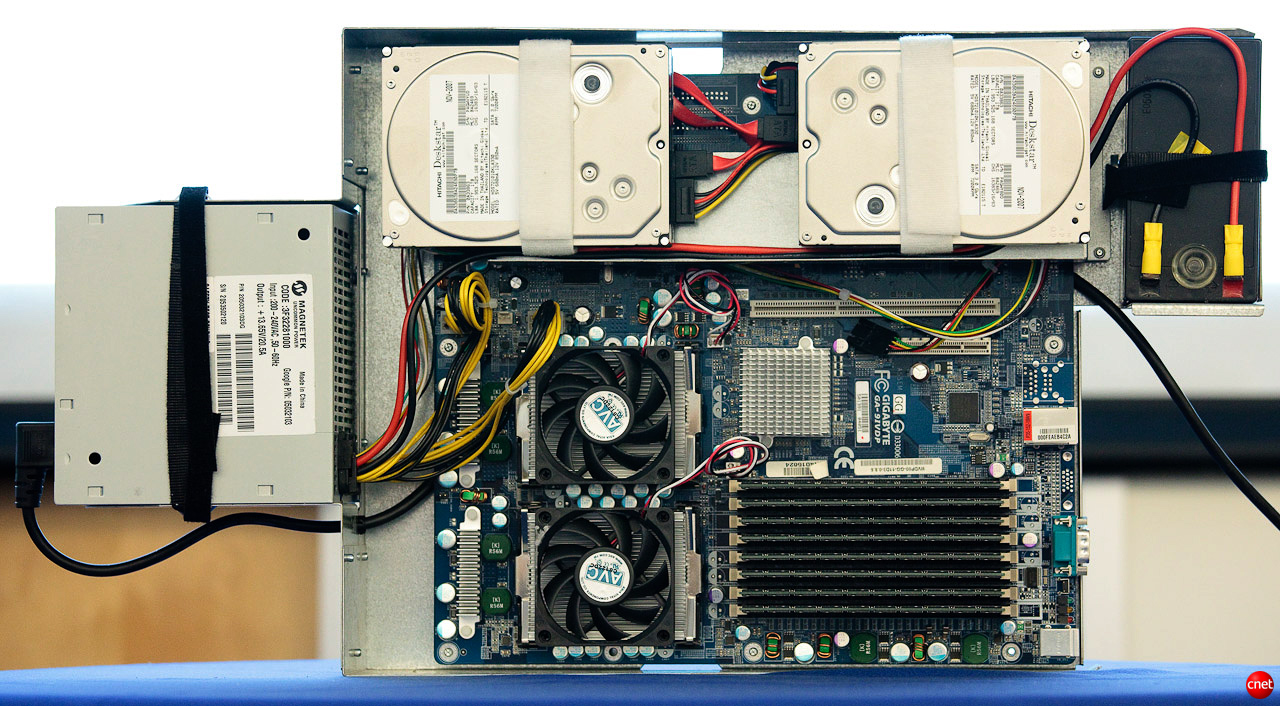
\includegraphics[width=0.83\textwidth]{images/GoogleServerLarge}
        \caption{First generation of custom Google server}
        \label{fig:google1stsrv}
    \end{minipage}%
    \begin{minipage}{0.5\textwidth}
        \centering
        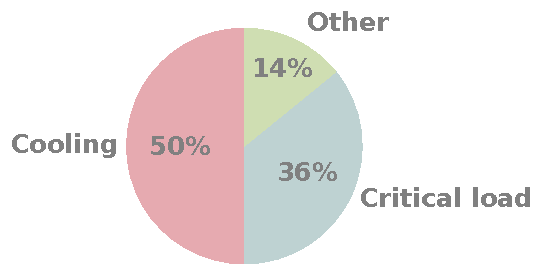
\includegraphics[width=0.9\textwidth]{images/power-pie.pdf}
        \caption{Data center power consumption}
        \label{fig:power-bd}
    \end{minipage}%
\end{figure}

We can offer great savings even when using stock, high-end, and expensive
servers such as the Dell T430 \cite{T430} that we use in our example. The problem
is that using stock servers is very expensive. Exactly as the TCO of the
traditional internal IT of Table \ref{table:clouds-comparison} is unrealistic
for companies such as Google and Amazon, the price of \SI{10641}[\$]{} for the
resources provided by our Dell T430 is also unrealistic for them. Google,
Amazon, and Facebook design and build their own hardware with total focus on
efficiency.

Google uses custom built servers for more than 10 years now, Figure
\ref{fig:google1stsrv} \cite{cnetgsrv} shows a Google server from 2006. Every
component of the Google server is there to minimize the TCO, including the open
case, and the battery. Following the efficiency masters, we will design, build,
and sell our own high-end low cost hardware, which will be the next step in
reducing costs of connected computing resources for our customers, helping them
to be more competitive.

\subsection{Electrical Efficiency} 
\label{subsec:ee}

% Describe how your innovation will contribute to any substantial impact
% addressing issues related to climate change or the environment, or bring other
% important benefits to society.

The \textit{iWe} decentralized architecture doesn't require the equipment
density of a typical data center, which is an opportunity to reduce power
consumption with cooling. In a typical data center only 36\% of power is used
for the critical load such as servers and networking equipment, cooling alone
consume 50\%, and the remaining 14\% are consumed by other important loads
\cite{apc-dc-power}.  Figure \ref{fig:power-bd} illustrates a breakdown of how
electricity is consumed among the various loads in a typical data center
\cite{apc-dc-power}. The lower server density of \textit{iWe} architecture is
an opportunity to save up to 50\% in power consumption, which has very positive
environmental impact.

If we opted for the typical data center approach for our small scale deployment,
we would install all our notebooks in a single location, which would require
using a small air conditioning unit. This air conditioning unit would at least
match the power consumption of our notebooks\footnote{All power that is consumed
by IT equipment is converted to heat. Though power is typically reported in
watts (W) and heat is typically reported in British Thermal Units (BTUs), these
units are in fact interchangeable \cite{cisco-dc-power}.}, multiplying by two
the total power consumption of our small scale deployment. However we are going
to use our distributed architecture, and we will install our notebooks in 20
different locations, which will not require the addition of per-location cooling
systems.  Our architecture allows us to save 50\% in power consumption compared
to the typical data center approach.

\subsection{Commercial Potential}
\label{subsec:company}

% How does the innovation project fit with the strategy of the participating
% SME(s)

% What is the relevance and rationale of the innovation project for the
% management team of the SME (or lead SME(s) in a consortium)

% What is the expected growth potential of your solution in terms of turnover,
% employment, market seize, IP management, sales, return on investment and
% profit etc.

While the SME \textit{iWe Provider} of our example get cloud resources 15
times cheaper, we make \SI{23040}[\$]{} in 3 years with the provision of our
services.  There is a long road ahead of us before our services are ready for
the market, but our business model and cloud architecture suggest that we will
offer an exceptional service with low operational costs. We have to carefully
define metrics before making reasonable financial estimations, but we can make
an educated guess based on our example SME \textit{iWe Provider}.  This
customer gives us \SI{640}[\$]{} per month, but we can make an estimation based
on 33\% of that value. If we make \SI{214}[\$]{} per month per \textit{iWe
Provider}, we can reach a monthly turnover of \SI{1}[\$]{M} with less than 5000
customers:

\begin{equation}
    \SI{1}[\$]{M}_{turnover} = \frac{\SI{1000000}[\$]{}}{\SI{214}[\$]{}} = 4673~Customers
\end{equation}

We believe it is feasible to have 5000 small \textit{iWe Providers} in our
first year of operation. 5000 customers is 0.005\% of the estimated 1M public
cloud customers Amazon had in the end of 2015 \cite{howlongaws}. And we expect
to be able to handle the first 5000 \textit{iWe Provider} customers with a
team of approximately 25 employees. We also expect that the number of
\textit{iWe Providers} per \textit{iWe} employee will increase with scale,
reducing our expenses per customer.
 % Section II
%\clearpage
%\input{implementation2} % Section III

%\backmatter
%\subfile{clalld-h2020-stage1-part2}
%\input{members} % Section IV
%\input{ethics} % Section V
%\appendix
%\clearpage
%% Proposal appendix
\vspace{15ex} % label
\chapter{Appendix}
\label{cha:appendix}

See Section \ref{sec:positioning} for background information.

This section shows benchmark results that were collected over a period of 30
days for Network, CPU, Memory, IO, and two data bases. The tests were executed
every 5 minutes to collect sustainable performance results, and we were careful
to not show the performance of our small iWe provider under a favorable light,
mainly for the IO tests.

We used a batch of simultaneous HTTPS transfers for bandwidth, and the sysbench
tool with two running threads for CPU, memory and IO. For the database tests we
used a customized version of the benchmark tools from the LevelDB project. The
source code is available on
github\footnote{https://github.com/petersenna/leveldb}.

The iWe provider we are evaluated had two home-grade servers, each with 16GB of
RAM, two SSD disks in RAID-1 and an i5-3320M CPU. The provider is connected to
the Internet over a 1Gbps fiber link. While this configuration is very small, it
allowed us to demonstrate that we can get similar levels of performance on the
lower end of the hardware spectrum.

\begin{figure}
\centering
\begin{subfigure}{.5\textwidth}
  \centering
  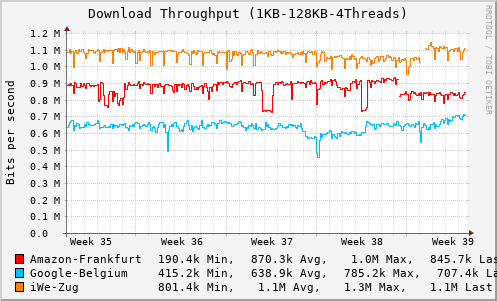
\includegraphics[width=0.98\textwidth]{30d-perf/download-month}
  \vspace{-0.05in}
  \caption{Download speed}
  \vspace{0.1in}
  \label{fig:sub1}
\end{subfigure}%
\begin{subfigure}{.5\textwidth}
  \centering
  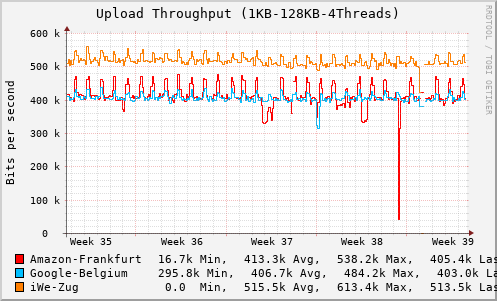
\includegraphics[width=0.98\textwidth]{30d-perf/upload-month}
  \vspace{-0.05in}
  \caption{Upload speed}
  \vspace{0.1in}
  \label{fig:sub2}
\end{subfigure}
\begin{subfigure}{.5\textwidth}
  \centering
  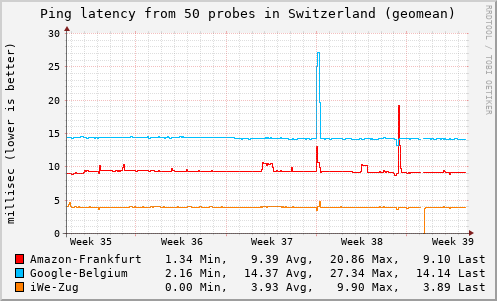
\includegraphics[width=0.98\textwidth]{30d-perf/ping-month}
  \vspace{-0.05in}
  \caption{Network latency}
  \vspace{0.1in}
  \label{fig:sub3}
\end{subfigure}%
\begin{subfigure}{.5\textwidth}
  \centering
  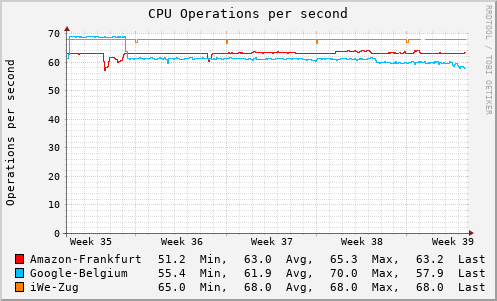
\includegraphics[width=0.98\textwidth]{30d-perf/cpu_ops-month}
  \vspace{-0.05in}
  \caption{Computing Power}
  \vspace{0.1in}
  \label{fig:sub4}
\end{subfigure}
\begin{subfigure}{.5\textwidth}
  \centering
  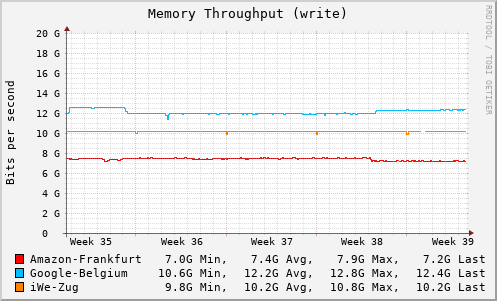
\includegraphics[width=0.98\textwidth]{30d-perf/mem_write-month}
  \vspace{-0.05in}
  \caption{Memory bandwidth}
  \vspace{0.1in}
  \label{fig:sub5}
\end{subfigure}%
\begin{subfigure}{.5\textwidth}
  \centering
  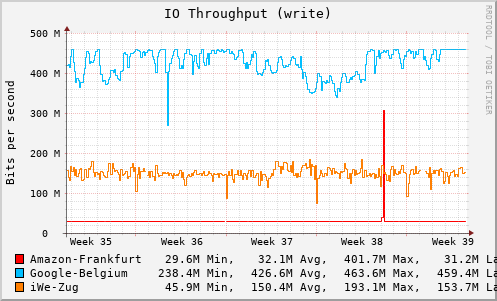
\includegraphics[width=0.98\textwidth]{30d-perf/io_write-month}
  \vspace{-0.05in}
  \caption{IO bandwidth}
  \vspace{0.1in}
  \label{fig:sub6}
\end{subfigure}
\begin{subfigure}{.5\textwidth}
  \centering
  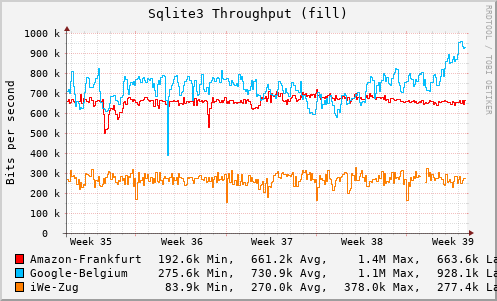
\includegraphics[width=0.98\textwidth]{30d-perf/sqlite3_fill-month}
  \vspace{-0.05in}
  \caption{SQLite3 write performance}
  \vspace{0.1in}
  \label{fig:sub7}
\end{subfigure}%
\begin{subfigure}{.5\textwidth}
  \centering
  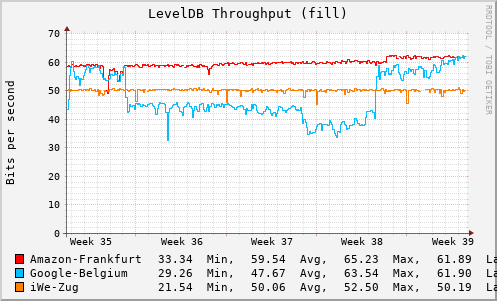
\includegraphics[width=0.98\textwidth]{30d-perf/leveldb_fill-month}
  \vspace{-0.05in}
  \caption{LevelDB write performance}
  \vspace{0.1in}
  \label{fig:sub8}
\end{subfigure}
  \caption{Performance Graphs}
  \label{graphs}
\end{figure}
\clearpage
 % Appendix
\bibliographystyle{plain}%
\bibliography{refs}%
\end{document}
